\input{preambolo_comune}

\title{Cifrari a Blocchi}
\author{Basato sulle slide della Prof.ssa Jocelyne Elias}
\date{\today}

\begin{document}

\maketitle
\tableofcontents
\newpage

\section{Block Ciphers (Cifrari a Blocchi)}

I cifrari a blocchi sono algoritmi crittografici che operano su blocchi di dati di dimensione fissa.

\subsection{Concetti Fondamentali}
\begin{itemize}
    \item \textbf{Funzionamento Generale}:
    \begin{itemize}
        \item Un blocco di testo in chiaro (Plaintext - PT) di $n$ bit viene trasformato in un blocco di testo cifrato (Ciphertext - CT) della stessa dimensione ($n$ bit).
        \item Questa trasformazione (E per Encryption, D per Decryption) dipende da una chiave segreta (Key) di $k$ bit.
    \end{itemize}
\end{itemize}

\begin{figure}[H]
\centering
\begin{tikzpicture}[node distance=3cm, auto, every node/.style={text=primarytext}]
    \node [ioblock, text width=3cm] (pt) {PT Block ($n$ bit)};
    \node [block, text width=2cm, right=3cm of pt] (ed) {E, D};
    \node [keyblock, text width=2cm, below=2cm of ed] (key) {Key};
    \node [ioblock, text width=3cm, right=3cm of ed] (ct) {CT Block ($n$ bit)};

    \draw [dataline] (pt) -- (ed);
    \draw [dataline] (ed) -- (ct);
    \draw [keyline] (key) -- node[right, xshift=0.1cm, text=white] {$k$ bits} (ed);
\end{tikzpicture}
\caption{Schema base di un cifrario a blocchi.}
\end{figure}

\begin{itemize}
    \item \textbf{Esempi Canonici} (dimensione blocco $n$, dimensione chiave $k$):
    \begin{itemize}
        \item \textbf{DES (Data Encryption Standard)}: $n = 64$ bit (8 byte), $k = 56$ bit
        \item \textbf{3DES (Triple DES)}: $n = 64$ bit, $k = 168$ bit (3 chiavi DES)
        \item \textbf{AES (Advanced Encryption Standard)}: $n = 128$ bit, $k = 128, 192, \text{o } 256$ bit
    \end{itemize}
    \item \textbf{Costruzione Iterativa}:
    \begin{itemize}
        \item Molti cifrari a blocchi moderni sono costruiti iterando una \textbf{funzione di round} per un certo numero di volte ($I$).
        \item \textbf{Key Expansion}: La chiave master $k$ viene espansa in sotto-chiavi di round ($k_1, k_2, \dots, k_I$).
        \item \textbf{Processo}: $m_i = R(k_i, m_{i-1})$, dove $m_0$ è il plaintext $m$, e $c = m_I$.
    \end{itemize}
\end{itemize}

\begin{figure}[H]
\centering
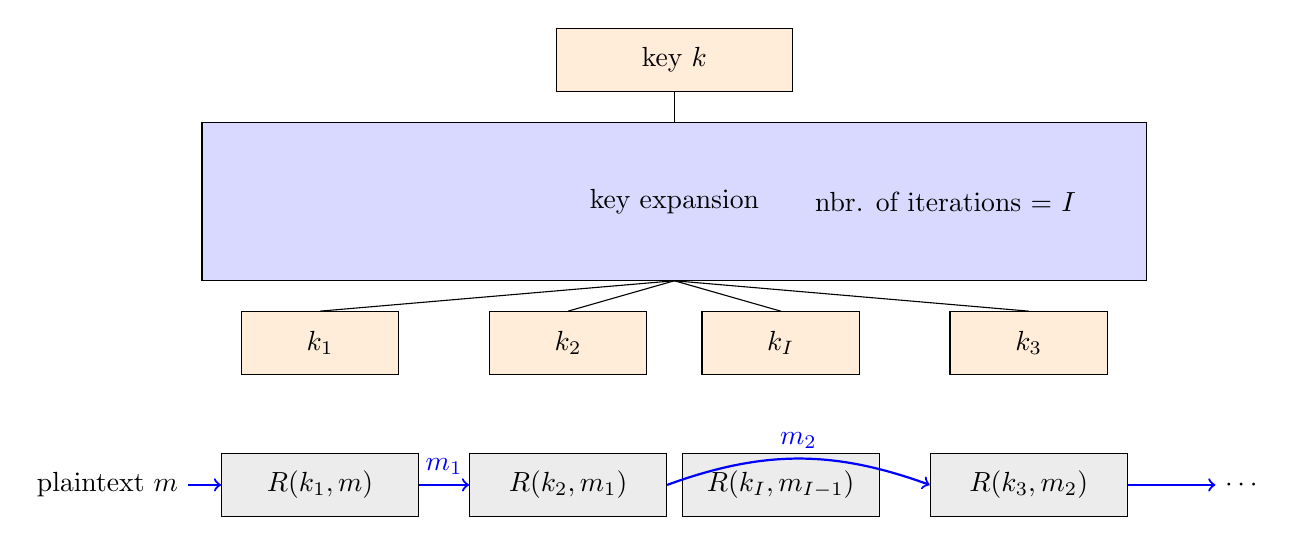
\begin{tikzpicture}[
    scale=0.9,
    box/.style={draw, rectangle, minimum width=2cm, minimum height=1cm},
    key/.style={draw, fill=orange!15, minimum width=2cm, minimum height=0.8cm},
    round/.style={draw, fill=gray!15, minimum width=2.5cm, minimum height=0.8cm}
]
    % Key k at top
    \node[key, minimum width=3cm] (key) at (0,0) {key $k$};
    
    % Key expansion box
    \node[box, fill=blue!15, minimum width=12cm, minimum height=2cm] (expansion) at (0,-2) {key expansion};
    \node[anchor=east] at (5.8,-2) {nbr. of iterations = $I$};
    
    % Key boxes below expansion
    \node[key] (k1) at (-5,-4) {$k_1$};
    \node[key] (k2) at (-1.5,-4) {$k_2$};
    \node[key] (kI) at (1.5,-4) {$k_I$};
    \node[key] (k3) at (5,-4) {$k_3$};
    
    % Round function boxes
    \node[round] (r1) at (-5,-6) {$R(k_1,m)$};
    \node[round] (r2) at (-1.5,-6) {$R(k_2,m_1)$};
    \node[round] (rI) at (1.5,-6) {$R(k_I,m_{I-1})$};
    \node[round] (r3) at (5,-6) {$R(k_3,m_2)$};
    
    % Input and dots
    \node (input) at (-8,-6) {plaintext $m$};
    \node (dots) at (8,-6) {$\cdots$};
    
    % Vertical connections from expansion to keys
    \foreach \x in {k1,k2,kI,k3}
        \draw[-] (expansion.south) -- (\x.north);
    
    % Horizontal data flow with proper path routing
    \draw[blue, thick, ->] (input) -- (r1);
    \draw[blue, thick, ->] (r1.east) -- node[above] {$m_1$} (r2.west);
    \draw[blue, thick, ->] (r2.east) to[bend left=20] node[above] {$m_2$} (r3.west);
    \draw[blue, thick, ->] (r3.east) -- (dots);
    
    % Key to expansion connection
    \draw[-] (key.south) -- (expansion.north);

\end{tikzpicture}
\caption{Cifrario a blocchi costruito per iterazione.}
\end{figure}


\subsection{Performance}
Generalmente, i cifrari a blocchi possono essere più lenti dei cifrari a flusso.
\begin{table}[H]
\centering
\caption{Performance Ciphers (Crypto++ 5.6.0, AMD Opteron, 2.2 GHz, Linux)}
\begin{tabular}{|l|l|l|c|}
\hline
\rowcolor{bg_custom}
\textbf{Tipo}   & \textbf{Cipher} & \textbf{Block/Key Size (bits)} & \textbf{Speed (MB/sec)} \\ \hline
Stream & RC4           & -                              & 126                     \\
Stream & Salsa20/12    & -                              & 643                     \\
Stream & Sosemanuk     & -                              & 727                     \\ \hline
Block  & 3DES          & 64/168                         & 13                      \\
Block  & AES-128       & 128/128                        & 109                     \\ \hline
\end{tabular}
\label{tab:perf}
\end{table}
\textit{Nota}: Le performance dipendono dall'implementazione e dall'hardware.


\section{Data Encryption Standard (DES)}

\subsection{Storia e Contesto}
\begin{itemize}
    \item \textbf{Primi anni '70}: Horst Feistel progetta \textit{Lucifer} presso IBM (chiave 128 bit, blocco 128 bit).
    \item \textbf{1973}: NBS (ora NIST) richiede proposte per un cifrario a blocchi standard.
    \item \textbf{1976}: NBS adotta DES come standard federale:
    \begin{itemize}
        \item Lunghezza chiave: \textbf{56 bit}
        \item Lunghezza blocco: \textbf{64 bit}
    \end{itemize}
    \item \textbf{1997}: DES "rotto" tramite ricerca esaustiva (brute-force). Problema: chiave troppo corta.
    \item \textbf{2000}: NIST adotta Rijndael come AES per sostituire DES.
\end{itemize}

\subsection{Idea Centrale: Rete di Feistel (Feistel Network)}
DES è basato su una Rete di Feistel. Permette di costruire una funzione invertibile partendo da funzioni di round $f_i$ non necessariamente invertibili.
\begin{itemize}
    \item \textbf{Input}: Blocco da 64 bit diviso in $L_0$ (32 bit) e $R_0$ (32 bit).
    \item \textbf{Per ogni round $i$ (da 1 a $d=16$ per DES)}:
    \begin{itemize}
        \item $L_i = R_{i-1}$
        \item $R_i = L_{i-1} \oplus f_i(R_{i-1}, k_i)$ (dove $f_i$ è la funzione di round con sotto-chiave $k_i$)
    \end{itemize}
    \item \textbf{Invertibilità}: La decifratura usa la stessa struttura, ma con sotto-chiavi in ordine inverso.
        \begin{itemize}
            \item $R_{i-1} = L_i$
            \item $L_{i-1} = R_i \oplus f_i(R_{i-1}, k_i) = R_i \oplus f_i(L_i, k_i)$
        \end{itemize}
\end{itemize}
\textit{Nota}: AES \textbf{non} usa una rete di Feistel.

\begin{figure}[H]
    \centering
    \begin{tikzpicture}[
        scale=0.9,
        node distance=2cm and 3cm,
        % Define styles
        block/.style={rectangle, draw=black, thick, fill=white, minimum width=2cm, minimum height=1cm, text=black},
        round/.style={circle, draw=black, thick, fill=white, minimum size=0.8cm, text=black},
        input/.style={rectangle, draw=black, thick, fill=gray!10, minimum width=1.8cm, minimum height=0.8cm, text=black},
        output/.style={rectangle, draw=black, thick, fill=gray!20, minimum width=1.8cm, minimum height=0.8cm, text=black},
        arrow/.style={->, thick, black}
    ]
    
    % Input nodes (left side)
    \node (Lin) [input] at (0,2) {$L_{i-1}$};
    \node (Rin) [input] at (0,0) {$R_{i-1}$};
    
    % Function block
    \node (f) [block] at (4,0) {$f_i$};
    
    % XOR operation
    \node (xor) [round] at (4,2) {$\oplus$};
    
    % Output nodes (right side)
    \node (Lout) [output] at (8,2) {$L_i$};
    \node (Rout) [output] at (8,0) {$R_i$};
    
    % Arrows - clean and logical flow
    % R_{i-1} goes straight to L_i
    \draw [arrow] (Rin.east) -- (6,0) |- (Lout.west);
    
    % R_{i-1} also goes to function f_i
    \draw [arrow] (Rin.east) -- (f.west);
    
    % L_{i-1} goes to XOR
    \draw [arrow] (Lin.east) -- (xor.west);
    
    % f_i output goes to XOR
    \draw [arrow] (f.north) -- (xor.south);
    
    % XOR output goes to R_i
    \draw [arrow] (xor.east) -- (Rout.west);
    
    % Labels for bit width
    \node [above=0.3cm of Lin, text=black] {$n$ bits};
    \node [above=0.3cm of Rin, text=black] {$n$ bits};
    \node [above=0.3cm of Lout, text=black] {$n$ bits};
    \node [above=0.3cm of Rout, text=black] {$n$ bits};
    
    % Key input to function (optional - can be removed if not needed)
    \node [above=0.5cm of f, text=black] {$k_i$};
    \draw [arrow] (4,1) -- (f.north);
    
    % Clean equations below
    \node [below=1.5cm of Rin, align=left, text=black] {
        \textbf{Feistel Round:}\\[0.3cm]
        $L_i = R_{i-1}$\\[0.2cm]
        $R_i = L_{i-1} \oplus f_i(R_{i-1}, k_i)$
    };
    
    \end{tikzpicture}
    \caption{Feistel Network Round (Input: $L_{i-1}, R_{i-1}$ $\rightarrow$ Output: $L_i, R_i$)}
    \label{fig:feistel_round}
\end{figure}

\subsection{Struttura Generale di DES}
\begin{enumerate}
    \item \textbf{Permutazione Iniziale (IP)}: Sul blocco di input da 64 bit.
    \item \textbf{16 Round di Feistel}: Ciascuno con una sotto-chiave da 48 bit.
    \item \textbf{Scambio delle Metà}: Dopo il 16° round, $L_{16}$ e $R_{16}$ vengono scambiate.
    \item \textbf{Permutazione Finale (IP$^{-1}$)}: Inversa di IP.
\end{enumerate}
\begin{itemize}
    \item \textbf{Lunghezza Chiave Effettiva}: 56 bit (64 bit nominali, ma 8 sono di parità).
\end{itemize}

\subsection{Generazione delle Sotto-Chiavi ($K_1 - K_{16}$)}
Dalla chiave master da 56 bit (dopo aver scartato i bit di parità):
\begin{enumerate}
    \item \textbf{Permuted Choice 1 (PC-1)}: La chiave da 64 bit è permutata e ridotta a 56 bit effettivi (scartando i bit di parità: 8, 16, ..., 64).
    \item \textbf{Divisione}: I 56 bit sono divisi in $C_0$ (28 bit) e $D_0$ (28 bit).
    \item \textbf{Per ogni round $i$ (da 1 a 16)}:
    \begin{itemize}
        \item $C_i, D_i$ sono ottenuti da $C_{i-1}, D_{i-1}$ tramite \textbf{shift circolare a sinistra (LS)}.
        \begin{itemize}
            \item Shift di \textbf{1 posizione} per i round 1, 2, 9, 16.
            \item Shift di \textbf{2 posizioni} per gli altri round.
        \end{itemize}
        \item \textbf{Permuted Choice 2 (PC-2)}: Dai 56 bit ($C_i || D_i$) vengono selezionati e permutati \textbf{48 bit} per formare la sotto-chiave $K_i$.
    \end{itemize}
\end{enumerate}
PC-1 e PC-2 sono tabelle di permutazione fisse definite nello standard.

\subsection{Chiavi Deboli (Weak Keys) in DES}
\begin{itemize}
    \item DES ha 4 chiavi deboli. Causano la generazione di sotto-chiavi identiche o pattern ripetitivi (es. $K_1 = K_2 = \dots = K_{16}$).
    \item Esempi: `0101010101010101` (hex), `FEFEFEFEFEFEFEFE` (hex).
    \item Riducono la sicurezza. Evitabili in fase di generazione.
\end{itemize}

\subsection{Permutazione Iniziale (IP) e Finale (IP$^{-1}$)}
Tabelle fisse che rimescolano i bit. Non aggiungono sicurezza crittografica.
Ad esempio, per IP: il 1° bit dell'output proviene dal 58° bit dell'input.

\subsection{La Funzione $f(k_i, R_{i-1})$ (Funzione di Round DES)}
Input: 32 bit da $R_{i-1}$, sotto-chiave $k_i$ da 48 bit. Output: 32 bit.
\begin{enumerate}
    \item \textbf{Espansione (E)}: I 32 bit di $R_{i-1}$ sono espansi a 48 bit (duplicando e permutando alcuni bit tramite tabella E).
    \item \textbf{XOR con Sotto-Chiave}: I 48 bit espansi $\oplus$ $k_i$.
    \item \textbf{S-box (Substitution boxes)}:
    \begin{itemize}
        \item I 48 bit sono divisi in 8 blocchi da 6 bit.
        \item Ogni blocco da 6 bit entra in una \textbf{S-box} specifica ($S_1, \dots, S_8$).
        \item Ogni S-box (tabella di lookup) prende 6 bit $\rightarrow$ 4 bit.
        \begin{itemize}
            \item Input 6 bit: $b_1 b_2 b_3 b_4 b_5 b_6$.
            \item Riga: $b_1 b_6$ (2 bit esterni).
            \item Colonna: $b_2 b_3 b_4 b_5$ (4 bit centrali).
        \end{itemize}
        \item Output totale: $8 \times 4 = 32$ bit.
        \item \textbf{Le S-box forniscono non-linearità e sono il cuore della sicurezza di DES}.
    \end{itemize}
    \item \textbf{Permutazione (P)}: I 32 bit dalle S-box sono permutati (tabella P) per diffusione.
\end{enumerate}

\begin{figure}[H]
\centering
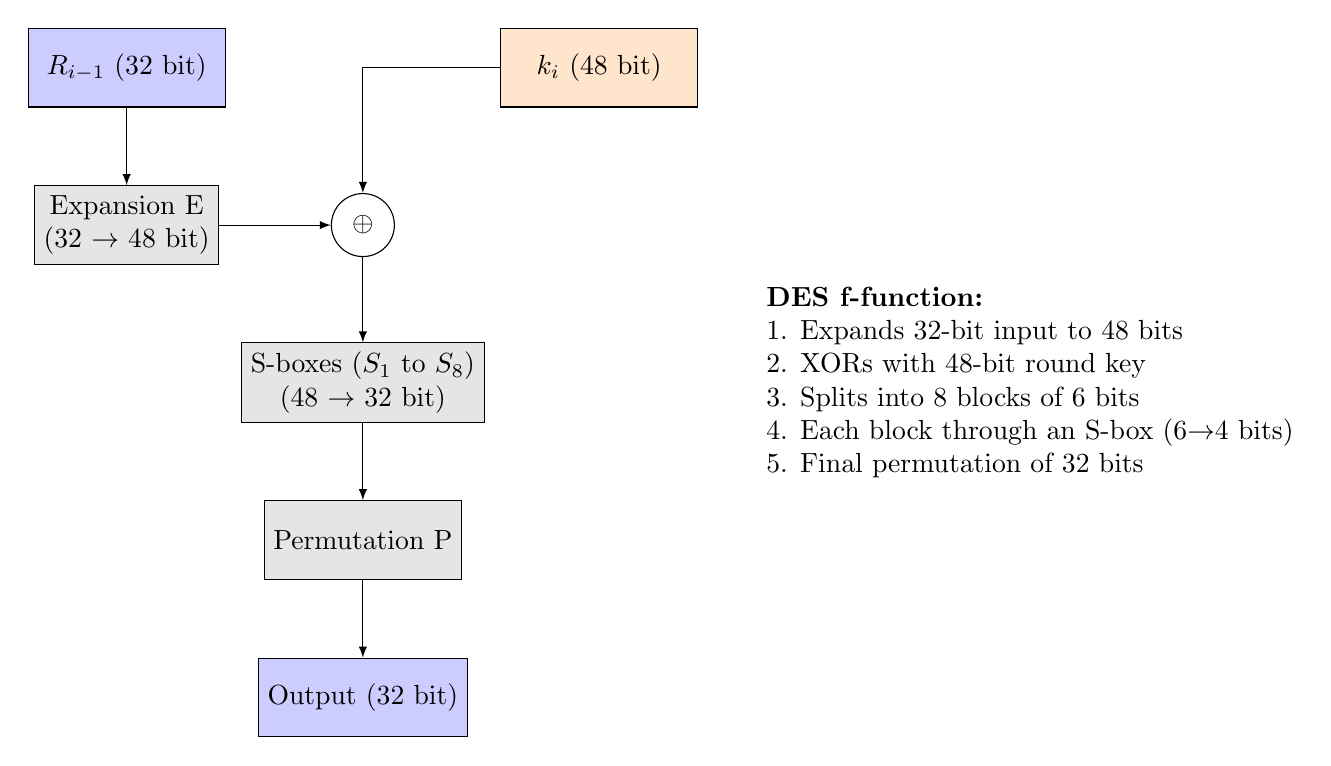
\begin{tikzpicture}[
    node distance=1.5cm,
    box/.style={draw, rectangle, minimum width=2cm, minimum height=1cm, fill=gray!20},
    iobox/.style={draw, rectangle, minimum width=2.5cm, minimum height=1cm, fill=blue!20},
    keybox/.style={draw, rectangle, minimum width=2.5cm, minimum height=1cm, fill=orange!20},
    xor/.style={circle, draw, minimum size=0.8cm},
    >=latex
]
    % Input and key nodes
    \node[iobox] (input) at (0,0) {$R_{i-1}$ (32 bit)};
    \node[keybox] (key) at (6,0) {$k_i$ (48 bit)};
    
    % Expansion box
    \node[box, align=center] (expand) at (0,-2) {Expansion E\\(32 $\rightarrow$ 48 bit)};
    
    % XOR operation
    \node[xor] (xor) at (3,-2) {$\oplus$};
    
    % S-boxes (simplified representation)
    \node[box, align=center] (sboxes) at (3,-4) {S-boxes ($S_1$ to $S_8$)\\(48 $\rightarrow$ 32 bit)};
    
    % Permutation box
    \node[box] (perm) at (3,-6) {Permutation P};
    
    % Output
    \node[iobox] (output) at (3,-8) {Output (32 bit)};
    
    % Arrows
    \draw[->] (input) -- (expand);
    \draw[->] (expand) -- (xor);
    \draw[->] (key) -| (xor);
    \draw[->] (xor) -- (sboxes);
    \draw[->] (sboxes) -- (perm);
    \draw[->] (perm) -- (output);
    
    % Add explanatory text on the right
    \node[align=left, anchor=west] at (8,-4) {
        \textbf{DES f-function:}\\
        1. Expands 32-bit input to 48 bits\\
        2. XORs with 48-bit round key\\
        3. Splits into 8 blocks of 6 bits\\
        4. Each block through an S-box (6$\rightarrow$4 bits)\\
        5. Final permutation of 32 bits
    };
\end{tikzpicture}
\caption{Simplified structure of the DES f-function.}
\end{figure}

\subsection{Effetto Valanga (Avalanche Effect)}
Piccolo cambiamento in input (PT o chiave) $\rightarrow$ grande cambiamento in output (CT, circa metà dei bit). DES esibisce un buon effetto valanga.

\subsection{Ricerca Esaustiva della Chiave}
\begin{itemize}
    \item \textbf{Obiettivo}: Dati $(m_i, c_i)$, trovare $k$ t.c. $c_i = \text{DES}(k, m_i)$.
    \item Chiave 56 bit $\implies 2^{56}$ (circa $7.2 \times 10^{16}$) chiavi possibili.
    \item \textbf{Unicità della chiave}: Con 1 coppia $(m,c)$, prob. chiave unica $\approx 99.5\%$. Con 2 coppie, prob. molto più alta. \textbf{Due coppie (PT,CT) sono sufficienti}.
    \item \textbf{DES Challenge}:
    \begin{itemize}
        \item 1998: EFF "Deep Crack" machine - \textbf{3 giorni}.
        \item 1999: Ricerca combinata - \textbf{22 ore}.
    \end{itemize}
    \item \textbf{Conclusione}: Chiavi a 56 bit sono troppo corte.
\end{itemize}

\begin{table}[H]
\centering
\caption{Tempo medio per ricerca esaustiva (dalla slide, valori indicativi)}
\begin{tabular}{|c|c|c|c|c|}
\rowcolor{bg_custom}
\hline
\textbf{Key Size} & \textbf{Cipher} & \textbf{Alternative Keys} & \textbf{Time @ $10^9$ dec/s} & \textbf{Time @ $10^{13}$ dec/s} \\ \hline
56 bits  & DES        & $\approx 7.2 \times 10^{16}$ & $\approx 1.125$ years & $\approx 1$ hour \\
128 bits & AES        & $\approx 3.4 \times 10^{38}$ & $\approx 5.3 \times 10^{21}$ years & $\approx 5.3 \times 10^{17}$ years \\
168 bits & Triple DES & $\approx 3.7 \times 10^{50}$ & $\approx 5.8 \times 10^{33}$ years & $\approx 5.8 \times 10^{29}$ years \\
\hline
\end{tabular}
\end{table}


\section{Rafforzare DES Contro la Ricerca Esaustiva}

\subsection{Double DES (2DES)}
\begin{itemize}
    \item $C = E_{k_1}(E_{k_2}(P))$. Chiave apparente: 112 bit.
    \item Decifrazione: $P = D_{k_2}(D_{k_1}(C))$.
    \item \textbf{Attacco Meet-in-the-Middle (MitM)}:
    \begin{itemize}
        \item Riduce la sicurezza a circa $2 \cdot 2^{56} = 2^{57}$ operazioni DES, con $2^{56}$ spazio di memoria.
        \item Dato $(m,c)$, si cerca $X$ t.c. $X = E_{k_2}(m)$ e $X = D_{k_1}(c)$.
        \item \textbf{Fase 1}: Per ogni $k_2$, calcola $X = E_{k_2}(m)$, memorizza $(X, k_2)$. Ordina per $X$.
        \item \textbf{Fase 2}: Per ogni $k_1$, calcola $Y = D_{k_1}(c)$, cerca $Y$ nella tabella. Se $Y=X$, $(k_1, k_2)$ è candidata.
    \end{itemize}
    \item 2DES offre solo un piccolo aumento di sicurezza.
\end{itemize}

\begin{figure}[H]
\centering
\begin{tikzpicture}[node distance=2cm and 1cm, every node/.style={text=primarytext}]
    \node (m) [ioblock] {$m$};
    \node (Ek2) [block, right=1.5cm of m, text width=3cm] {$E(k_2, \cdot)$};
    \node (intermediate) [circle, fill=red!70!black, minimum size=0.5em, right=1cm of Ek2, yshift=0cm, label={[yshift=-0.8cm, xshift=-0.2cm, color=red]:Meet Here}] {};
    \node (Ek1) [block, right=1cm of intermediate, text width=3cm] {$E(k_1, \cdot)$};
    \node (c) [ioblock, right=1.5cm of Ek1] {$c$};

    \draw [dataline] (m) -- (Ek2);
    \draw [dataline] (Ek2) -- (intermediate);
    \draw [dataline] (intermediate) -- (Ek1);
    \draw [dataline] (Ek1) -- (c);
\end{tikzpicture}
\caption{Attacco Meet-in-the-Middle su Double DES.}
\end{figure}

\subsection{Triple DES (3DES)}
\begin{itemize}
    \item Schema EDE: $C = E_{k_1}(D_{k_2}(E_{k_3}(P)))$. Chiavi $k_1, k_2, k_3$.
    \item Lunghezza chiave: $3 \times 56 = 168$ bit.
    \item Circa 3 volte più lento di DES.
    \item Se $k_1 = k_2 = k_3 \implies$ DES singolo.
    \item Attacco MitM: riduce forza effettiva a circa $2^{112}$ (non $2^{168}$). Slide indica tempo $2^{118}$, spazio $2^{56}$.
    \item 3DES è considerato sicuro contro brute-force sulla chiave.
\end{itemize}

\subsection{DESX}
\begin{itemize}
    \item $C = k_1 \oplus E_{k_2}(P \oplus k_3)$.
    \item $k_1, k_3$: chiavi di "whitening" da 64 bit. $k_2$: chiave DES 56 bit.
    \item Lunghezza chiave totale: $64+56+64 = 184$ bit.
    \item Aumenta complessità ricerca esaustiva (attacco in tempo $2^{64+56} = 2^{120}$ secondo slide).
    \item Posizione XOR cruciale: $k_1 \oplus E_{k_2}(P)$ o $E_{k_2}(P \oplus k_3)$ sono molto più deboli.
\end{itemize}

\section{Altri Attacchi sui Block Ciphers (DES)}

\subsection{Crittoanalisi Differenziale (Biham-Shamir)}
\begin{itemize}
    \item Attacco a testo in chiaro scelto.
    \item Si studiano le differenze XOR tra coppie di plaintext e i corrispondenti ciphertext ($\Delta P = P_1 \oplus P_2$, $\Delta C = C_1 \oplus C_2$).
    \item La distribuzione di $\Delta C$ dato $\Delta P$ può rivelare bit della sotto-chiave.
    \item \textbf{Resistenza di DES}:
    \begin{itemize}
        \item Gli autori di DES conoscevano questa tecnica; le S-box sono progettate per resistervi.
        \item Contro DES 16 round: richiede $2^{47}$ testi in chiaro scelti.
        \item \textbf{Non efficace contro DES completo in pratica}.
    \end{itemize}
\end{itemize}

\subsection{Crittoanalisi Lineare (Matsui, 1993)}
\begin{itemize}
    \item Attacco a testo in chiaro noto.
    \item Trova approssimazioni lineari del cifrario del tipo:
    $P[i_1] \oplus \dots \oplus C[j_1] \oplus \dots = K[l_1] \oplus \dots$
    che valga con probabilità $p \neq 0.5$.
    \item Sfrutta il bias statistico per dedurre bit della chiave.
    \item \textbf{Applicazione a DES}:
    \begin{itemize}
        \item DES 16 round: $2^{43}$ plaintext noti.
        \item \textbf{Non ha implicazioni pratiche contro DES completo} (troppi dati).
    \end{itemize}
\end{itemize}

\subsection{Attacchi all'Implementazione}
\begin{itemize}
    \item \textbf{Side Channel Attacks}: Osservano "effetti collaterali".
    \begin{itemize}
        \item Misura tempo, consumo di potenza (es. tracciato potenza DES su smartcard).
    \end{itemize}
    \item \textbf{Fault Attacks}: Induzione deliberata di errori.
    \begin{itemize}
        \item Errore nell'ultimo round può rivelare la chiave.
    \end{itemize}
    \item \textbf{Raccomandazione}: Non implementare primitive crittografiche da soli.
\end{itemize}

\section{Advanced Encryption Standard (AES)}

\subsection{Processo di Selezione AES}
\begin{itemize}
    \item \textbf{1997}: NIST richiede proposte per sostituire DES.
    \item \textbf{Requisiti}: Blocco 128 bit, chiavi 128, 192, 256 bit.
    \item \textbf{2000}: NIST sceglie \textbf{Rijndael} (Daemen, Rijmen - Belgio) come AES.
\end{itemize}

\subsection{Caratteristiche di AES}
\begin{itemize}
    \item \textbf{NON è un cifrario di Feistel}. È una \textbf{Substitution-Permutation Network (SPN)}.
    \item Efficiente in hardware e software.
    \item Opera iterativamente.
    \item \textbf{Parametri Fondamentali} (Standard AES FIPS 197):
\end{itemize}
\begin{table}[H]
\centering
\caption{Parametri AES}
\begin{tabular}{|l|c|c|c|}
\rowcolor{bg_custom}
\hline
\textbf{Versione} & \textbf{Key Length (Nk words)} & \textbf{Block Size (Nb words)} & \textbf{Number of Rounds (Nr)} \\ \hline
AES-128  & 4 (128 bit) & 4 (128 bit) & 10 \\
AES-192  & 6 (192 bit) & 4 (128 bit) & 12 \\
AES-256  & 8 (256 bit) & 4 (128 bit) & 14 \\ \hline
\end{tabular}
\label{tab:aes_params}
\newline \footnotesize{1 word = 32 bit. Nb è sempre 4 per lo standard AES.}
\end{table}
\begin{itemize}
    \item \textbf{Key Scheduling}: Genera $(Nr+1)$ sotto-chiavi da 128 bit.
\end{itemize}

\subsection{Sicurezza delle Chiavi AES}
\begin{itemize}
    \item AES-128: $2^{128} \approx 3.4 \times 10^{38}$ chiavi.
    \item AES-192: $2^{192} \approx 6.2 \times 10^{57}$ chiavi.
    \item AES-256: $2^{256} \approx 1.1 \times 10^{77}$ chiavi.
    \item Ricerca esaustiva infattibile. Considerato sicuro per molti anni.
\end{itemize}

\subsection{Struttura di AES (Substitution-Permutation Network - SPN)}
Applica trasformazioni all'intero blocco in ogni round.
\begin{figure}[H]
\centering
\begin{tikzpicture}[node distance=1.5cm and 0.7cm, every node/.style={text=primarytext}]
    \node (input) [ioblock, text width=1.5cm, minimum height=5em] {input};
    
    % Round 1
    \node (k1_add) [sum, right=of input, yshift=-1.5em] {$\oplus$};
    \node (k1_key) [keyblock, text width=1em, above=0.2cm of k1_add] {$k_1$};
    \node (s1_1) [block, text width=1.5em, right=of k1_add, yshift=1.5em] {$S_1$};
    \node (s1_2) [block, text width=1.5em, below=0.2cm of s1_1] {$S_2$};
    \node (s1_dots) [rotate=90, below=0.1cm of s1_2] {\dots};
    \node (s1_8) [block, text width=1.5em, below=0.1cm of s1_dots] {$S_N$}; % N instead of 8 for generality
    \node (perm1) [rectangle, draw=green, fill=green!20!black, minimum height=6em, minimum width=2em, right=0.5cm of s1_2, yshift=0.8em] {};
    \node at (perm1.center) [rotate=90, text=white] {Permutation};

    % Round 2
    \node (k2_add) [sum, right=0.8cm of perm1, yshift=0.8em] {$\oplus$};
    \node (k2_key) [keyblock, text width=1em, above=0.2cm of k2_add] {$k_2$};
    \node (s2_1) [block, text width=1.5em, right=of k2_add, yshift=1.5em] {$S_1$};
    \node (s2_2) [block, text width=1.5em, below=0.2cm of s2_1] {$S_2$};
    \node (s2_dots) [rotate=90, below=0.1cm of s2_2] {\dots};
    \node (s2_8) [block, text width=1.5em, below=0.1cm of s2_dots] {$S_N$};
    \node (perm2) [rectangle, draw=green, fill=green!20!black, minimum height=6em, minimum width=2em, right=0.5cm of s2_2, yshift=0.8em] {};
     \node at (perm2.center) [rotate=90, text=white] {Permutation};

    \node (dots_rounds) [right=0.5cm of perm2, yshift=0.8em] {\dots \dots};

    % Round r
    \node (kr_add) [sum, right=0.5cm of dots_rounds] {$\oplus$};
    \node (kr_key) [keyblock, text width=1em, above=0.2cm of kr_add] {$k_r$};
    \node (sr_1) [block, text width=1.5em, right=of kr_add, yshift=1.5em] {$S_1$};
    \node (sr_2) [block, text width=1.5em, below=0.2cm of sr_1] {$S_2$};
    \node (sr_dots) [rotate=90, below=0.1cm of sr_2] {\dots};
    \node (sr_8) [block, text width=1.5em, below=0.1cm of sr_dots] {$S_N$};
    
    \node (output) [ioblock, text width=1.5cm, minimum height=5em, right=0.5cm of sr_2, yshift=0.8em] {output};

    \draw[dataline] (input) -- (k1_add); \draw[keyline] (k1_key) -- (k1_add);
    \draw[dataline] (k1_add) -- (s1_1.west); \draw[dataline] (k1_add) -- (s1_2.west); \draw[dataline] (k1_add) -- (s1_8.west);
    \draw[dataline] (s1_1.east) -- (perm1.west |- s1_1.east);
    \draw[dataline] (s1_2.east) -- (perm1.west |- s1_2.east);
    \draw[dataline] (s1_8.east) -- (perm1.west |- s1_8.east);

    \draw[dataline] (perm1.east |- s2_1.west) -- (k2_add.west);
    \draw[keyline] (k2_key) -- (k2_add);
    \draw[dataline] (k2_add) -- (s2_1.west); \draw[dataline] (k2_add) -- (s2_2.west); \draw[dataline] (k2_add) -- (s2_8.west);
    \draw[dataline] (s2_1.east) -- (perm2.west |- s2_1.east);
    \draw[dataline] (s2_2.east) -- (perm2.west |- s2_2.east);
    \draw[dataline] (s2_8.east) -- (perm2.west |- s2_8.east);
    
    \draw[dataline] (perm2.east) -- (dots_rounds);
    \draw[dataline] (dots_rounds) -- (kr_add);
    \draw[keyline] (kr_key) -- (kr_add);
    \draw[dataline] (kr_add) -- (sr_1.west); \draw[dataline] (kr_add) -- (sr_2.west); \draw[dataline] (kr_add) -- (sr_8.west);
    \draw[dataline] (sr_1.east) -- (output.west |- sr_1.east);
    \draw[dataline] (sr_2.east) -- (output.west |- sr_2.east);
    \draw[dataline] (sr_8.east) -- (output.west |- sr_8.east);
    
    \node [below=0.5cm of input, text width=2cm, align=center] {Substitution layer};
    \node [below=1cm of perm1, text width=2cm, align=center, xshift=-0.5cm] {Permutation layer};

    \draw [->, draw=primarytext, thick, decorate, decoration={brace,amplitude=5pt,mirror}, xshift=0pt, yshift=0pt]
        ($(perm2.south east)+ (0.5cm, -1.2cm)$) -- ($(perm1.south west)+(-0.5cm, -1.5cm)$) node[midway,yshift=-0.5cm, text=primarytext] {Inversion for each step};

\end{tikzpicture}
\caption{AES come Substitution-Permutation Network (Schema generico).}
\end{figure}

\subsection{Processo di Cifratura AES}
Input: blocco 128 bit (16 byte) = matrice 4x4 \textbf{State}.
\begin{enumerate}
    \item \textbf{KeyExpansion}.
    \item \textbf{InitialRound (AddRoundKey)}: State $\oplus$ prima sotto-chiave.
    \item \textbf{Rounds ($N_r-1$ volte)}:
    \begin{enumerate}
        \item \textbf{SubBytes()}: Sostituzione byte-byte (AES S-box).
        \item \textbf{ShiftRows()}: Shift ciclico delle righe.
        \item \textbf{MixColumns()}: Mixing lineare sulle colonne.
        \item \textbf{AddRoundKey()}: State $\oplus$ sotto-chiave del round.
    \end{enumerate}
    \item \textbf{FinalRound (1 volta)}: Senza MixColumns().
    \begin{enumerate}
        \item SubBytes()
        \item ShiftRows()
        \item AddRoundKey()
    \end{enumerate}
\end{enumerate}
Output: ciphertext.

\begin{figure}[H]
    \centering
    \begin{tikzpicture}[node distance=1cm and 0.5cm, scale=0.9, transform shape, every node/.style={text=primarytext}]
        \node (plaintext) [ioblock, text width=5cm] {Plaintext (16 bytes)};
        \node (add_key0) [block, text width=5cm, below=0.5cm of plaintext] {AddRoundKey (w[0-3])};
        \node (key_expand) [keyblock, text width=3cm, right=1cm of plaintext, yshift=-0.75cm] {Key (16 bytes) $\rightarrow$ Expand Key};
        \draw[keyline] (key_expand.south) -| (add_key0.east);
    
        % Define the round nodes first
        \node (sub_bytes1) [block, text width=5cm, below=0.8cm of add_key0] {SubBytes};
        \node (shift_rows1) [block, text width=5cm, below=0.5cm of sub_bytes1] {ShiftRows};
        \node (mix_cols1) [block, text width=5cm, below=0.5cm of shift_rows1] {MixColumns};
        \node (add_key1) [block, text width=5cm, below=0.5cm of mix_cols1] {AddRoundKey (w[4-7], etc.)};
        
        % Now define the box that fits around them
        \node (round1_box) [rectangle, draw=primarytext, rounded corners, fit=(sub_bytes1)(shift_rows1)(mix_cols1)(add_key1), inner sep=0.3cm, label={[xshift=0.4cm, yshift=-0.2cm, color=primarytext, font=\small]Round 1..$N_r-1$}] {};
        
        \draw[keyline] ($(key_expand.south) + (0,-1.5cm)$) -| (add_key1.east);
    
        \draw[dataline, very thick] (plaintext) -- (add_key0);
        \draw[dataline, very thick] (add_key0) -- (sub_bytes1);
        \draw[dataline, very thick] (sub_bytes1) -- (shift_rows1);
        \draw[dataline, very thick] (shift_rows1) -- (mix_cols1);
        \draw[dataline, very thick] (mix_cols1) -- (add_key1);
        
        \node (dots_rounds) [below=0.3cm of add_key1, yshift=-0.2cm, font=\Large] {$\vdots$};
    
        % Define the final round nodes first
        \node (sub_bytes_f) [block, text width=5cm, below=0.3cm of dots_rounds, yshift=-0.2cm] {SubBytes};
        \node (shift_rows_f) [block, text width=5cm, below=0.5cm of sub_bytes_f] {ShiftRows};
        % NO MixColumns in final round
        \node (add_key_f) [block, text width=5cm, below=0.5cm of shift_rows_f] {AddRoundKey (last w)};
        
        % Now define the final round box
        \node (final_round_box) [rectangle, draw=orange, rounded corners, fit=(sub_bytes_f)(shift_rows_f)(add_key_f), inner sep=0.3cm, label={[xshift=0.4cm, yshift=-0.2cm, color=orange, font=\small]Final Round ($N_r$)}] {};
        
        \draw[keyline] ($(key_expand.south) + (0,-4cm)$) -| (add_key_f.east);
    
        \draw[dataline, very thick] (add_key1) -- (dots_rounds);
        \draw[dataline, very thick] (dots_rounds) -- (sub_bytes_f);
        \draw[dataline, very thick] (sub_bytes_f) -- (shift_rows_f);
        \draw[dataline, very thick] (shift_rows_f) -- (add_key_f);
    
        \node (ciphertext) [ioblock, text width=5cm, below=0.5cm of add_key_f] {Ciphertext (16 bytes)};
        \draw[dataline, very thick] (add_key_f) -- (ciphertext);
    \end{tikzpicture}
    \caption{Schema della cifratura AES.}
    \end{figure}

\subsection{Trasformazioni di Round AES}
\begin{itemize}
    \item \textbf{SubBytes}: Sostituzione byte-byte (AES S-box, non-lineare).
    Ogni byte $A[i,j]$ dello State è sostituito con $S(A[i,j])$.
    \item \textbf{ShiftRows}: Shift ciclico a sinistra delle righe dello State (diffusione).
    \begin{itemize}
        \item Riga 0: no shift.
        \item Riga 1: shift di 1 byte.
        \item Riga 2: shift di 2 byte.
        \item Riga 3: shift di 3 byte.
    \end{itemize}
    \item \textbf{MixColumns}: Ogni colonna è moltiplicata per un polinomio fisso in GF($2^8$) (diffusione). \textbf{Non nell'ultimo round}.
    \item \textbf{AddRoundKey}: State $\oplus$ sotto-chiave di round.
\end{itemize}
Tutte le operazioni sono invertibili per la decifratura.

\subsection{Attacchi su AES}
AES è considerato molto sicuro.
\begin{itemize}
    \item \textbf{Miglior attacco di key recovery (2011)}: Complessità $\approx 2^{126}$ per AES-128. Ancora infattibile.
    \item \textbf{Attacco a Chiavi Correlate su AES-256 (2009)}:
    \begin{itemize}
        \item Richiede $2^{99}$ coppie input/output da \textbf{quattro chiavi correlate}. Tempo $\approx 2^{99}$.
        \item Considerato \textbf{non pratico} nella maggior parte degli scenari.
    \end{itemize}
\end{itemize}

\end{document}